\documentclass[../main.tex]{subfiles}
% DOCUMENT

\begin{document}

\chapter{Case study}\label{case-study}

Ngoài việc thử nghiệm với các dữ liệu sinh ngẫu nhiên, tôi còn sử dụng
thuật toán DDD cho bài toán MDP trên bộ dữ liệu thực tế từ mạng lưới
đường bộ Atlanta. Mạng này bao gồm 306 nút và 618 cung, được lấy từ Open
Street Map. \autoref{fig:14} mô tả bản đồ khu vực và biểu diễn mạng lưới tương
ứng.

\begin{figure}
\centering
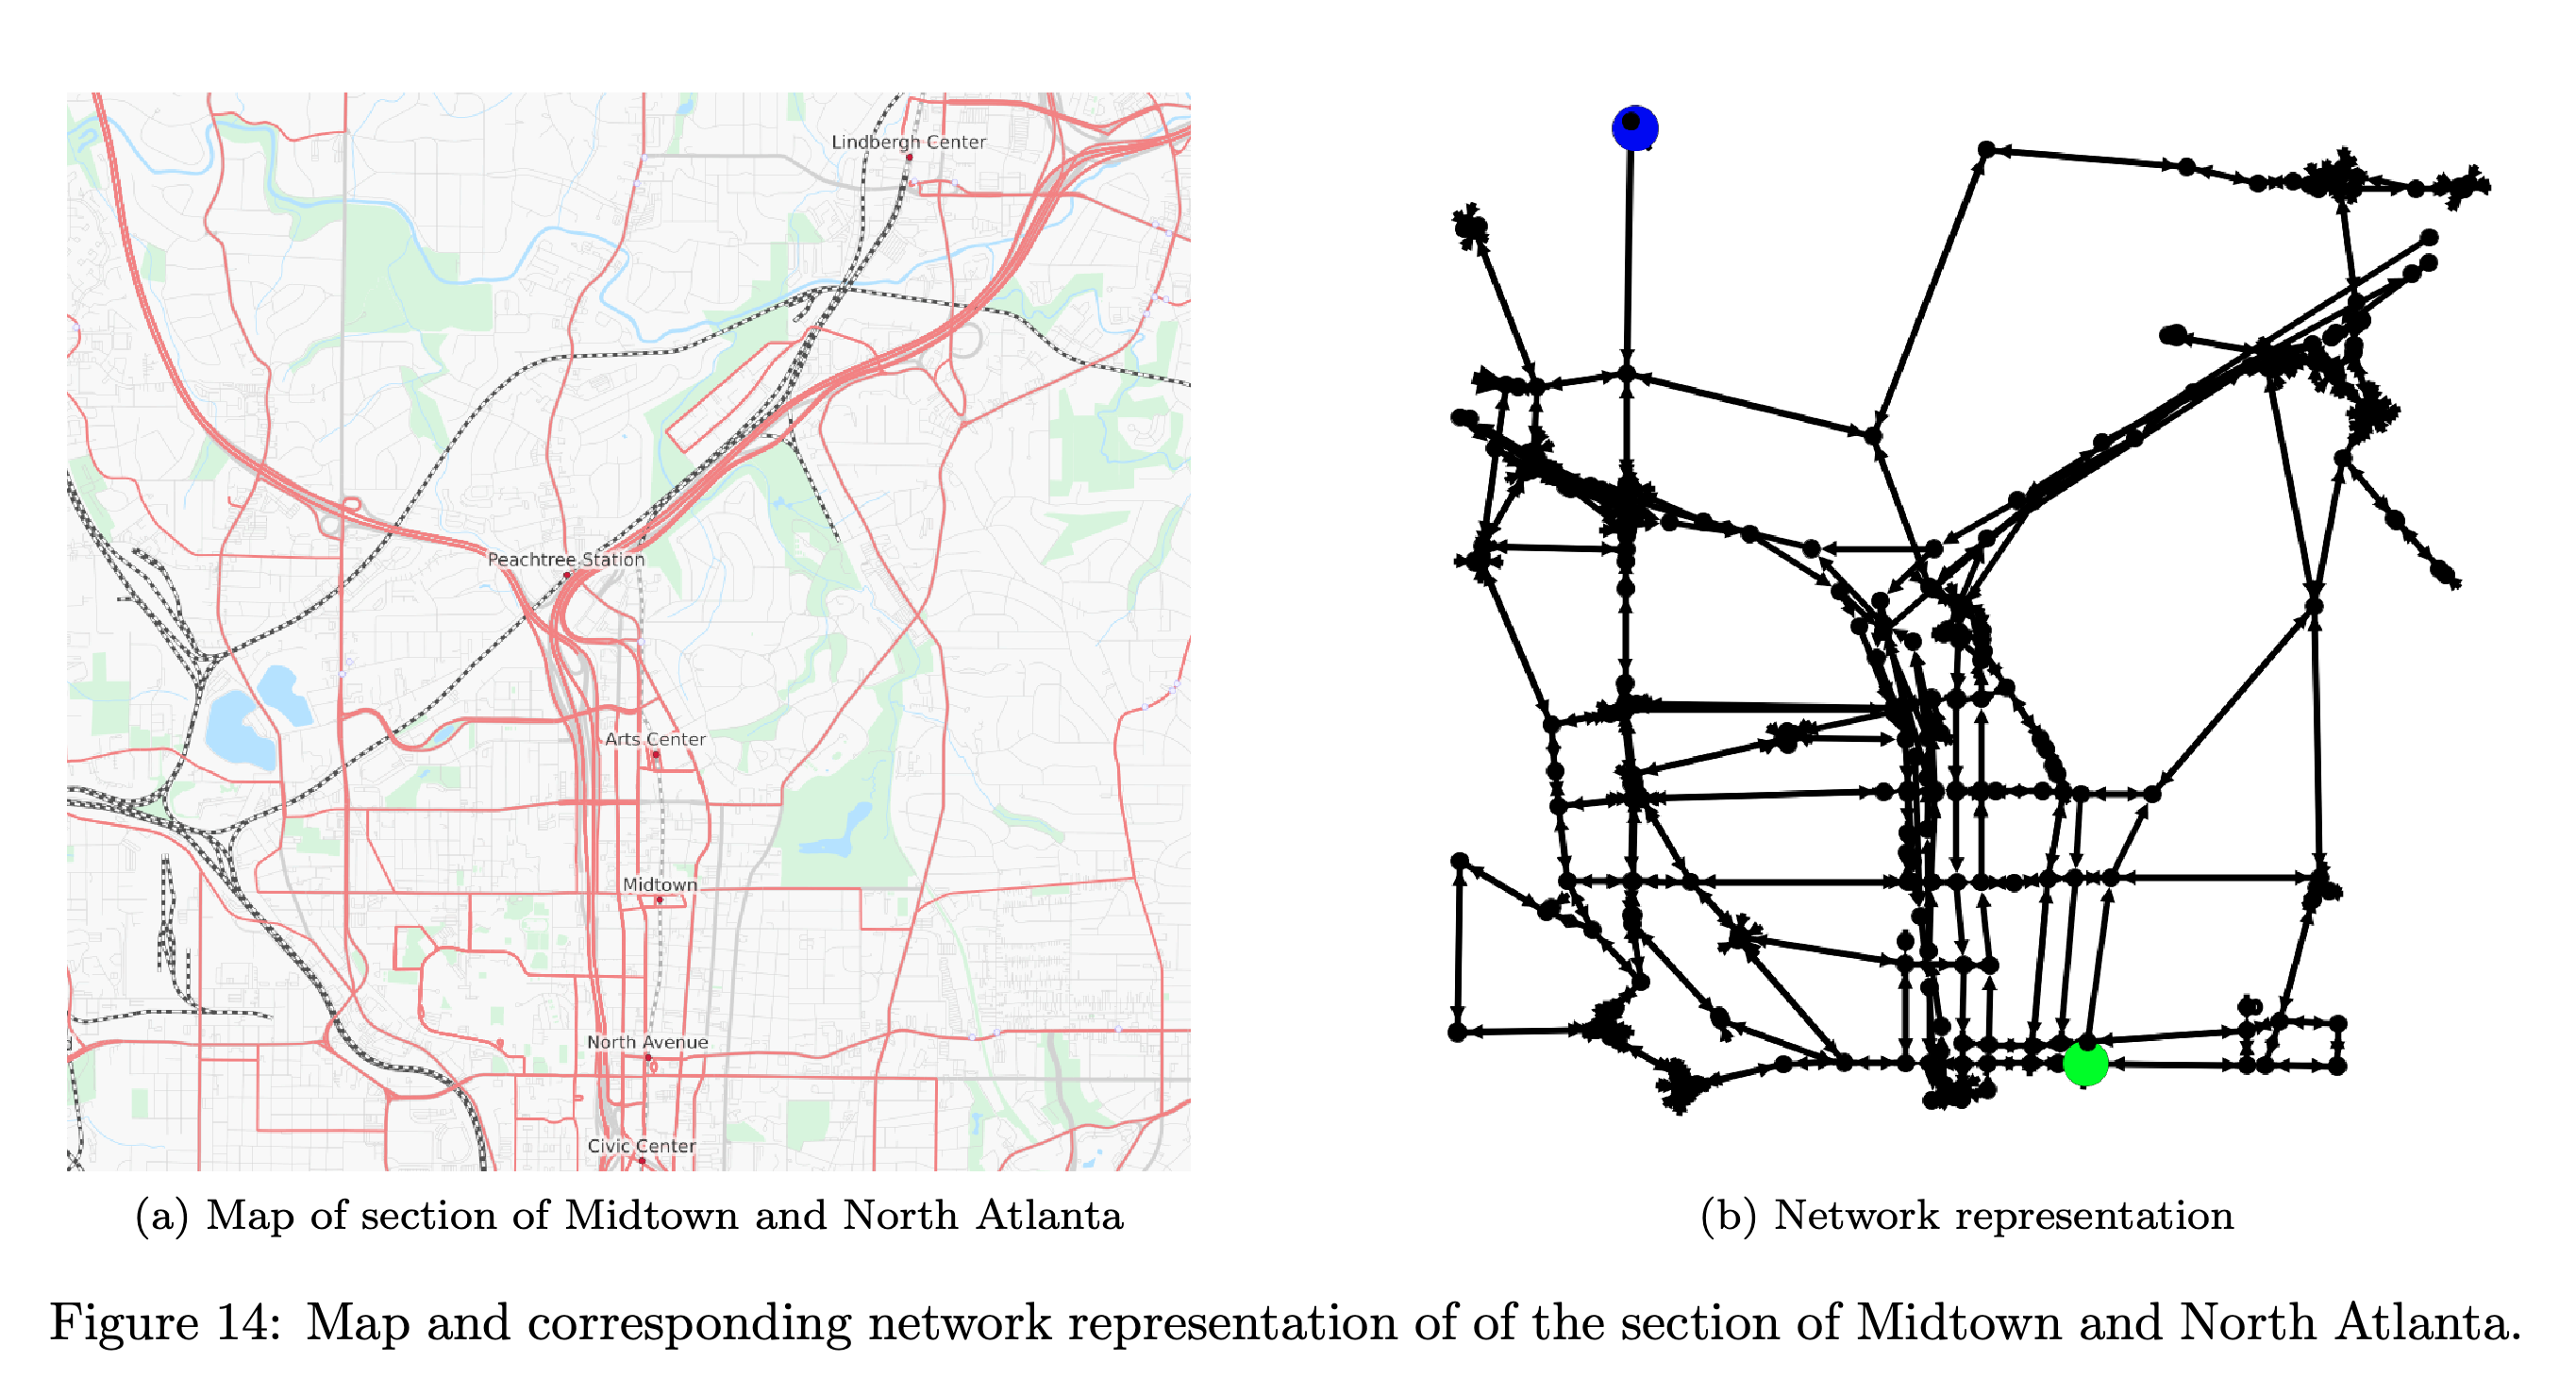
\includegraphics{images/Figure14.png}
\caption{Figure14}
\label{fig:14}
\end{figure}

Dữ liệu về thời gian di chuyển được thu thập từ nhiều nguồn khác nhau
(hệ thống định vị, dữ liệu di động). Dữ liệu được thu thập và tổng hợp
để tạo thành các hàm thời gian di chuyển tuyến tính từng khúc với các BP
cách nhau 15 phút trong 24 giờ. Nhờ vậy mỗi cung có tổng cộng 192 điểm
dữ liệu (Marshall 2019). \autoref{fig:15} là ví dụ về các hàm thời gian di chuyển
này.

\begin{figure}
\centering
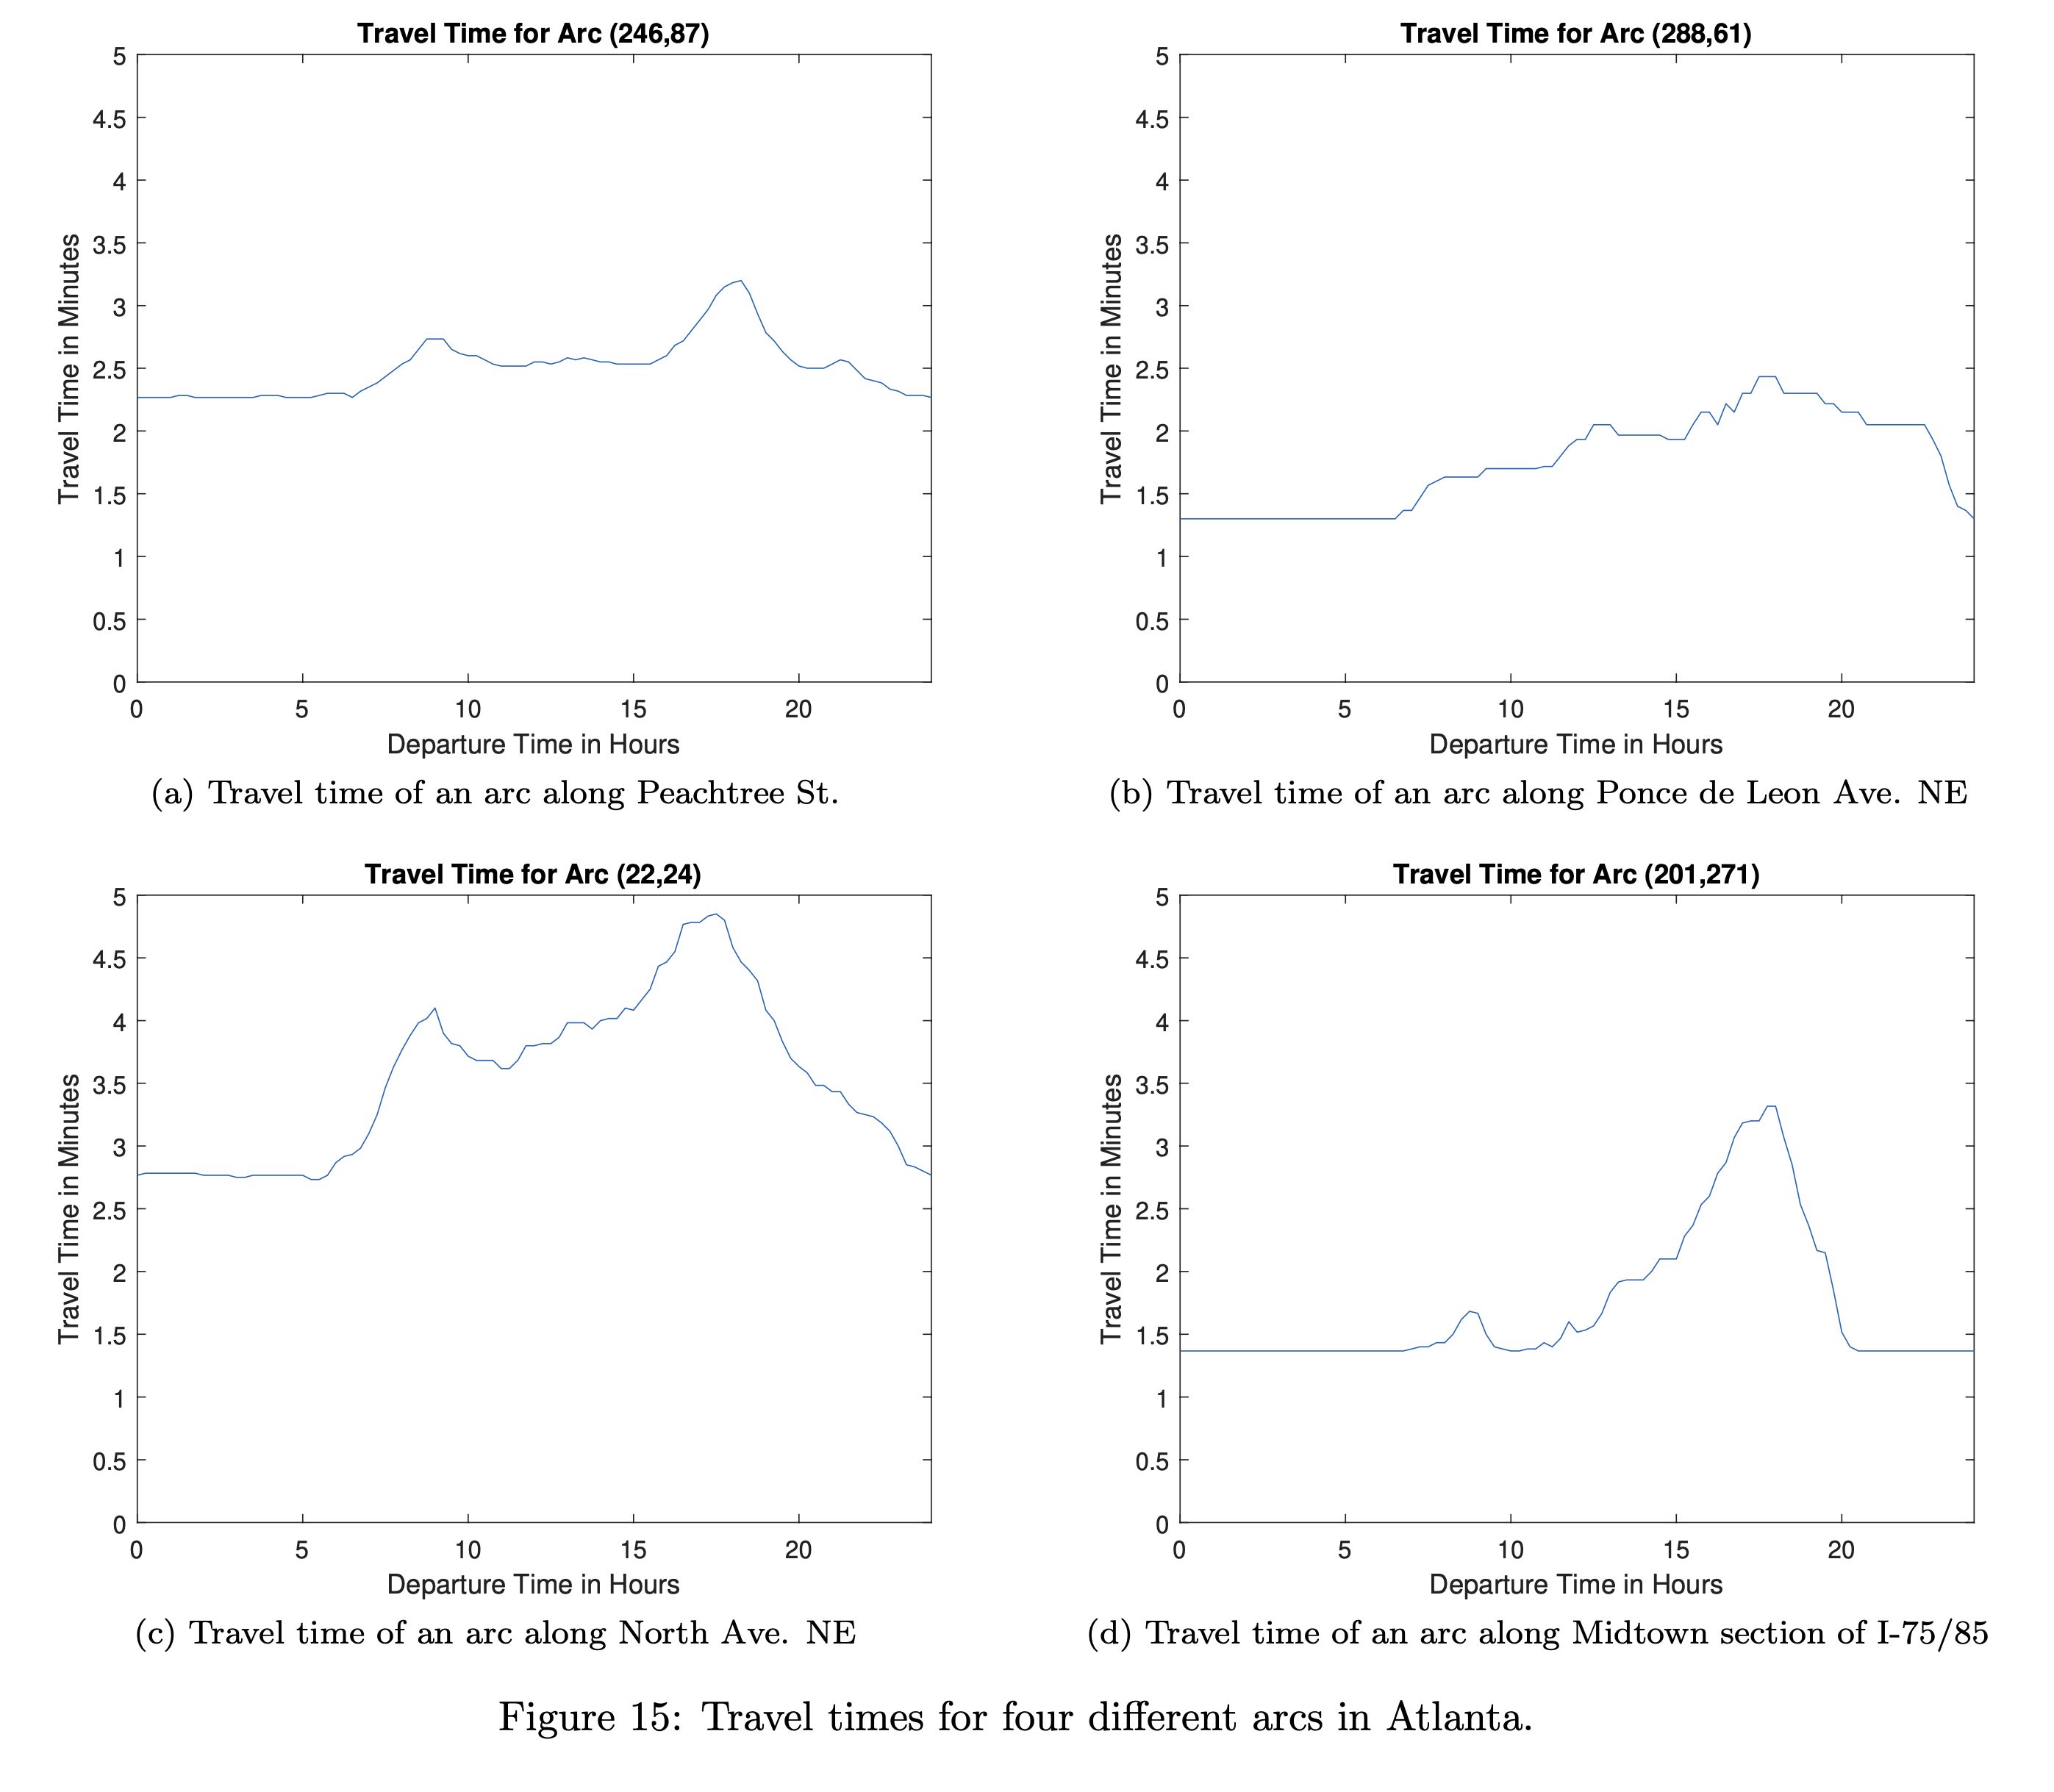
\includegraphics{images/Figure15.png}
\caption{Figure15}
\label{fig:15}
\end{figure}

Để minh hoạ sự khác biệt giữa đường đi tối thiểu thời gian thực hiện,
đến đích sớm nhất và khởi hành muộn nhất từ nguồn đến đích trong khoảng
thời gian cụ thể, tôi chọn điểm nguồn ở Bắc Atlanta, đích đến ở Trung
tâm Atlanta và khung thời gian là \([9:30, 13:00]\).

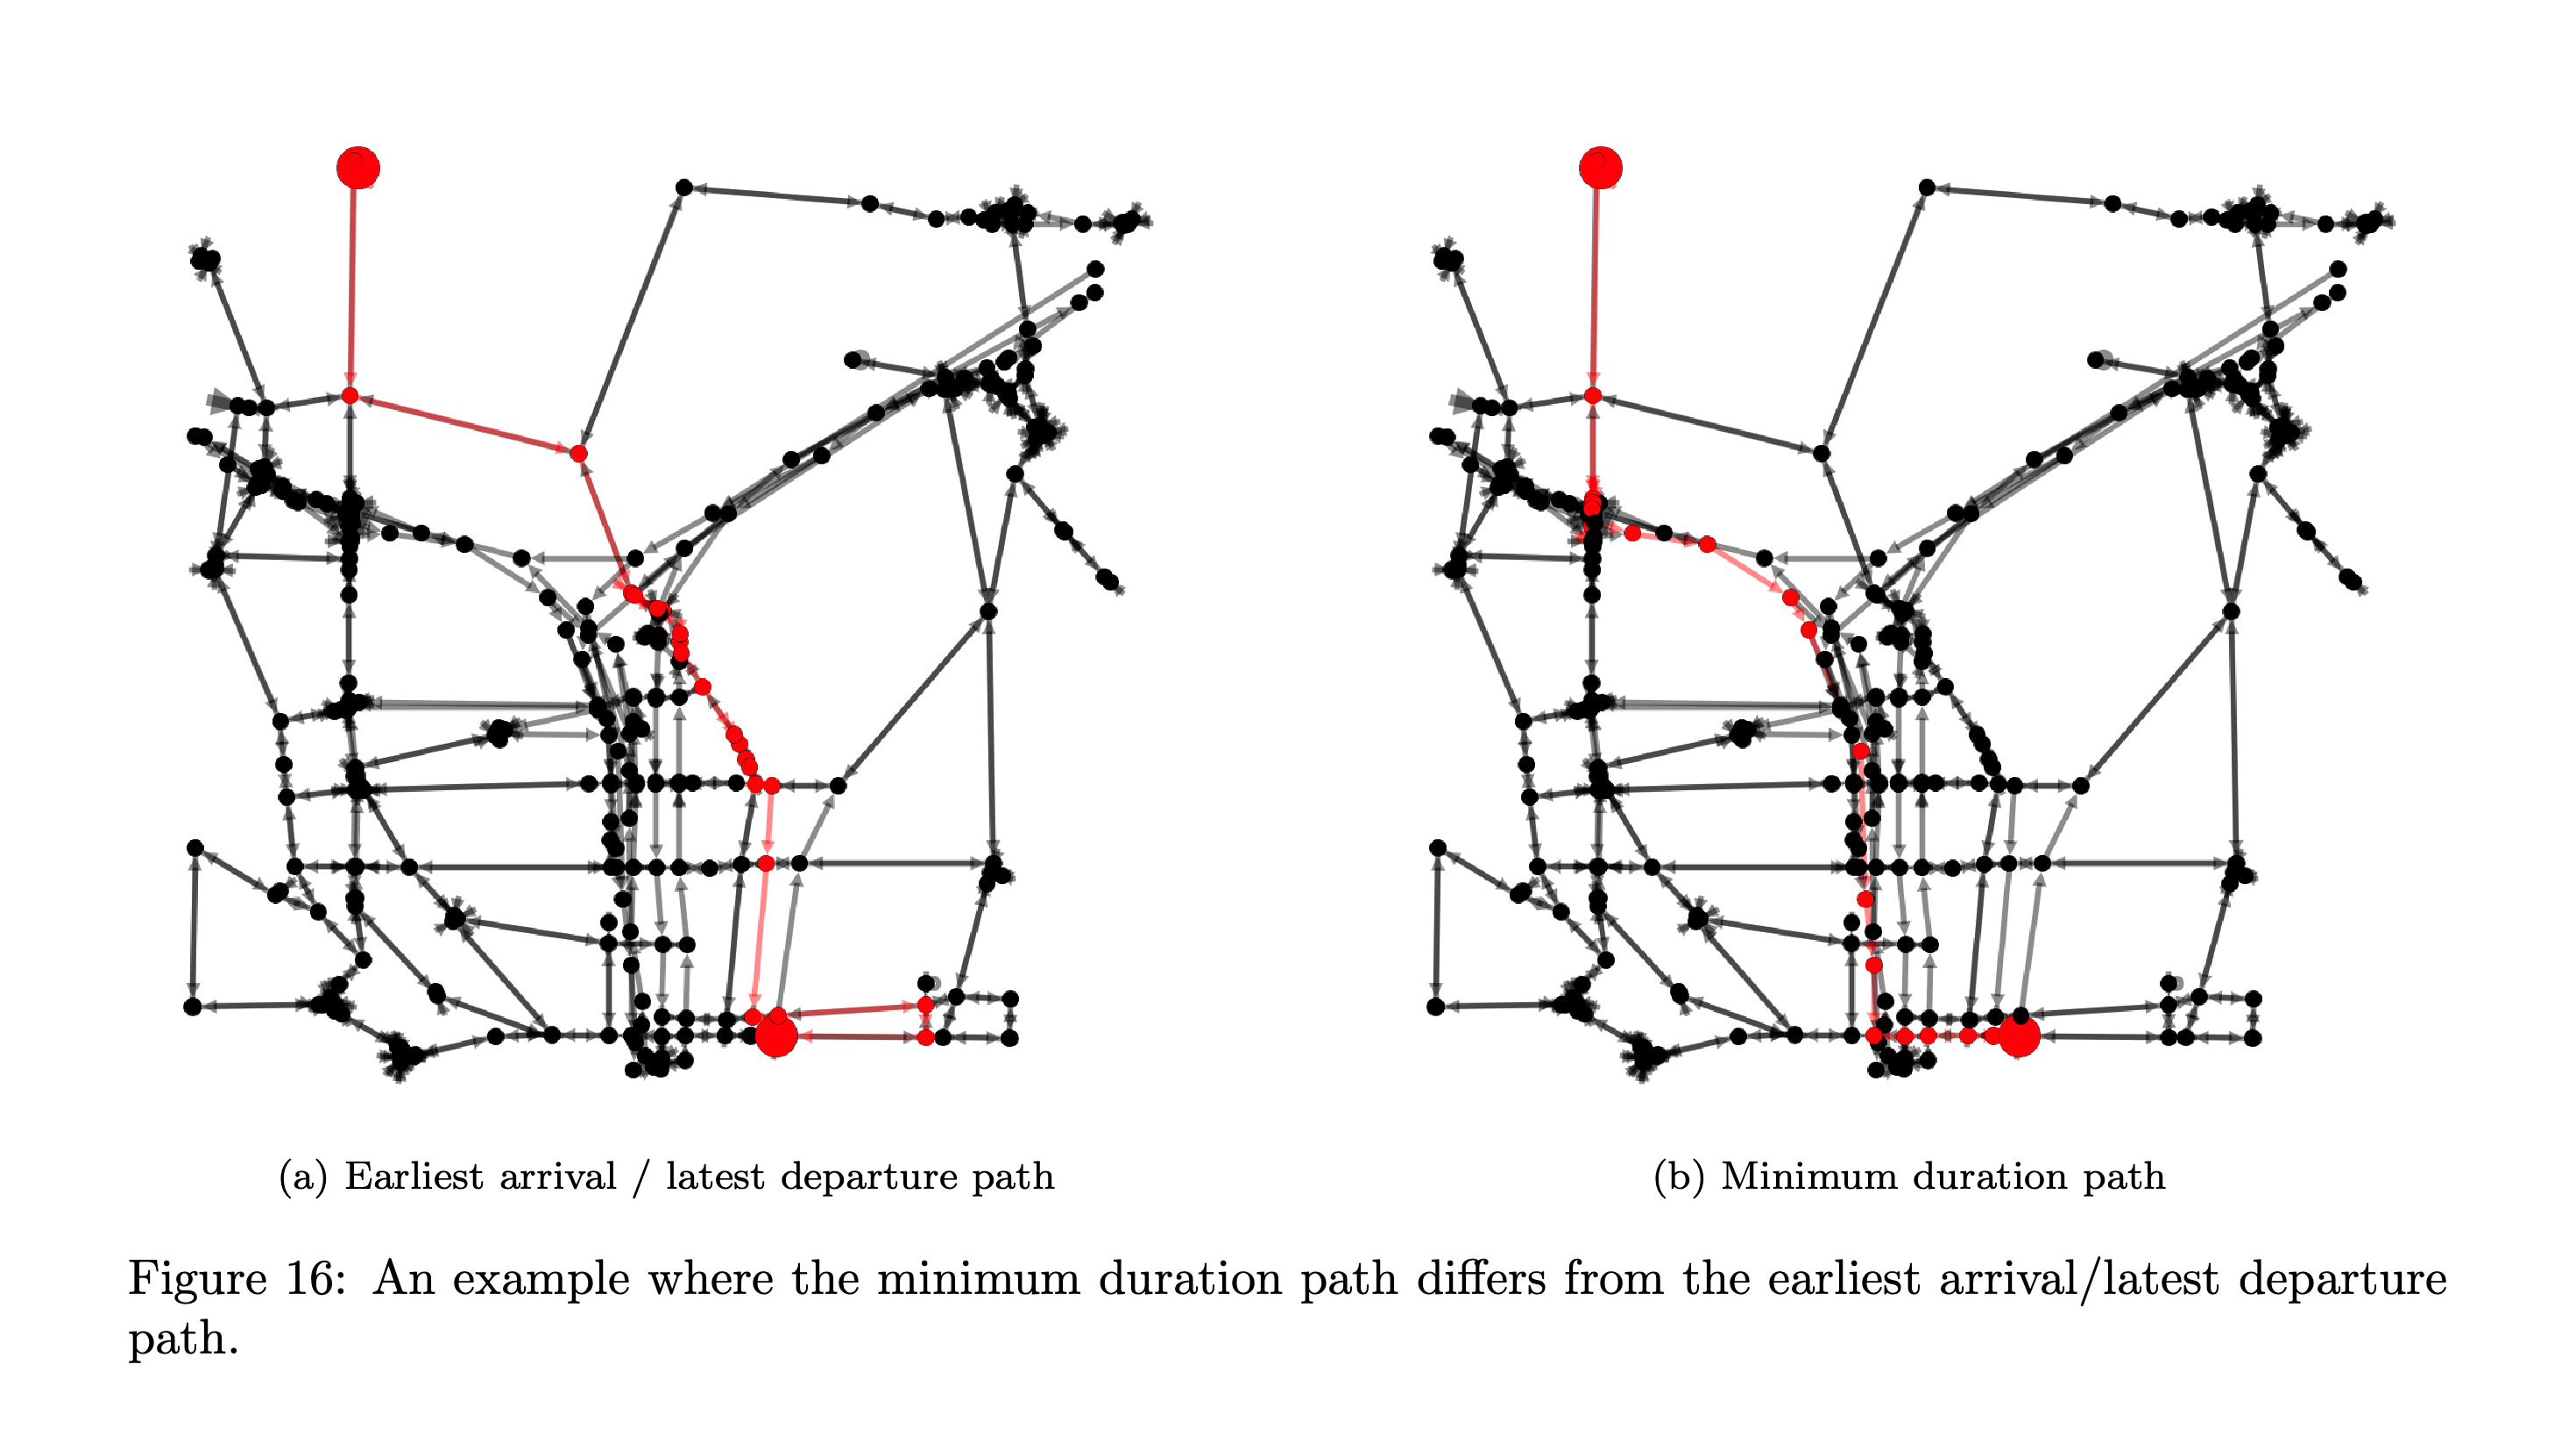
\includegraphics{images/Figure16.png} Đường đi tối thiểu thời gian thực
hiện (Hình 16(b)) xuất phát lúc \(10:37\) sáng và chỉ mất \(45.8\) phút,
trong khi đường đi đến đích sớm nhất mất \(47.5\) phút còn đường đi xuất
phát muộn nhất mất \(47.8\) phút (Hình 16(a)). Nguyên nhân cho sự khác
biệt này nằm ở việc đường đi tối thiểu thời gian khởi hành vào lúc vắng
xe (giữa giờ cao điểm sáng và trưa) và đi theo tuyến đường lớn nhất (cao
tốc \(I-75\) và \(I-75/85\)). Hai đường đi còn lại đi đường tránh cao
tốc, qua khu dân cư (Peachtree St.~và Juniper St.) và phải đi đường vòng
để tránh một chiều.

Mặc dù sự khác biệt trong thử nghiệm này không quá lớn (do khu vực
Atlanta được chọn khá bé và ít trường học), việc tìm đường đi chỉ mất
vài giây thời gian chạy. Điều này cho thấy phương pháp này có thể hữu
ích trong thực tế.
\backmatter
\end{document}
% END DOCUMENT